\section{Results}
To study the effects of multistability, non-linearities, boundary conditions, and growth, we use a simple reaction-diffusion model which consists of a 2-node Turing topology system with non-linear Hill-functions to represent gene activation and inhition.
The topology can be seen in Fig.~\ref{fig1}C where the activator $A$ activates itself and the inhibitor $I$, while the inhibitor $I$ inhibits the activator $A$:

\begin{subequations}
    \begin{equation}
        \pdv{[A]}{t}=b_{A}+V_{A} \cdot\frac{1}{1+\left(\frac{K_{AA}}{[A]}\right)^{n_{AA}}}\cdot\frac{1}{1+\left(\frac{[I]}{K_{IA}}\right)^{n_{IA}}}-\mu_{A}\cdot[A] + D_{A}\nabla^2 [A]
    \end{equation}


    \begin{equation}
        \pdv{[I]}{t}=\Underbrace{\textrm{basal production}}{b_{I}}+ \Underbrace{\textrm{regulated production}}{V_{I} \cdot\frac{1}{1+\left(\frac{K_{AI}}{[A]}\right)^{n_{AI}}}}-\Underbrace{\textrm{degradation}}{\mu_{I}\cdot[I]} +
        \Underbrace{\textrm{diffusion}}{D_{I}\nabla^2 [I]},
    \end{equation}

    \label{eq:turinghill}
\end{subequations}

with $\nabla^2=\partial^2/\partial x^2$ in 1D. The differential equations describe the rate of change in space and time as a combination of the basal production and regulated production, as well as degradation and diffusion. Parameter $b_{X}$ is the basal production rate which corresponds to the leakage of the promoter, producing molecules even when the system is fully inactivated. Furthermore, $V_{X}$ is the induced maximum production rate, $K_{XY}$ is the dissociation constant of X binding to Y regulator DNA, $n_{XY}$ is the Hill coefficient (cooperativity constant) of $X$ binding to the $Y$ regulator DNA, and $\mu_{X}$ is the linear degradation rate of $X$. Finally, $D_{X}$ is the diffusion constant of species $X$.

The boundary conditions and domain are not strictly defined here as they vary throughout the study. The boundary conditions used are   Neumann for reflective boundaries, where the derivative at the boundary is zero, as well as Dirilichet for absorbing boundaries, where the value at the boundary is zero.
The domain used is either a fixed domain of length $L$ or a linearly, isotropically and apically growing domain, which replicates the bacterial colony growth in 1D.



\subsection{Analytical to numerical: other types of dispersion relations and patterns} \label{nogrowth}

Turing instabilities are defined using linear stability analysis (LSA) (see Section~\ref{lsa}) as systems which are stable without diffusion, and become unstable as diffusion is introduced for a finite wavenumber. These Turing instabilities generally lead to stationary periodic patterns (see Fig.~\ref{fig:dispersions}B). In this section, we demonstrate how sometimes the classical Turing instability theory fails to predict pattern formation.
Other types of dispersion relations beyond classical Turing instabilities can produce stationary patterns and non-stationary regular patterns that might be of interest in developmental biology.

High-throughput studies like \cite{Scholes2019, Zheng2016, Marcon} only consider Turing I as patterning and the rest is discarded.
Here, we study solutions of the classical 2-node circuit (Fig.~\ref{fig1}C, Eq.~\ref{eq:turinghill} and explore beyond Turing I and stationary patterns to give a more complete view of the relationship between LSA and spatio-temporal patterns. 
First, LSA was carried out, as explained in Section \ref{lsa}, on particular parameter sets to find multiple steady states with different types of stability. 
Second, numerical simulations were computed using the Crank-Nicholson algorithm, where the initial condition is a random uniform distribution around a particular steady state.By classifying dispersion-relation types and pattern types, we document what type of dispersion relations in mono-stable systems can be linked to what type of patterns, to gain insights into predicting pattern formation from LSA. All the solutions used in this section are mono-stable systems to ensure a direct correlation between the dispersion relation and the pattern obtained.

All types of dispersion relations in our parameter space were classified into 5 types: stable dispersion relations have all eigenvalues $\sigma$ below zero for any wavenumber $k_{n}$ (Fig ~\ref{fig:dispersions}A). Unstable dispersion relations have a positive eigenvalue at $k_{0}=0$ which eventually drops below zero as diffusion is introduced, i.e. $k_{n}>0$ (Fig~\ref{fig:dispersions}C). Hopf-type dispersion relations, as with any unstable dispersion relation, show an instability without diffusion ($\sigma>0$ for $k_{0}=0$), which eventually drops below zero for positive wavenumbers. However, in the case of the Hopf-type dispersion relation, when the eigenvalues cross the zero line, there is a pair of complex conjugate eigenvalues (Fig~\ref{fig:dispersions}D).
A Hopf-like dispersion relation is different to a Hopf bifurcation: a bifurcation displays a shift in stability as a model parameter changes, while the Hopf-like dispersion is a change in stability as a function of the wavenumber $k_{n}$.
Turing I dispersion relations, as previously mentioned, are stable without diffusion, have an instability for a positive wavenumber, and finally become stable again for very large wavenumbers (Fig~\ref{fig:dispersions}B).
Turing I-Hopf dispersion relations, are a combination of Turing I and Hopf-type dispersion relations. As the Hopf-type dispersion, they are unstable without diffusion. Then, as $k_{n}$ is increased, the system becomes stable with a pair of complex conjugates as the eigenvalues cross the zero line.
Finally, a Turing I-type behaviour arises getting a peak above zero and decaying again for large wavenumbers (Fig~\ref{fig:dispersions}E).

Other types of dispersion relation exist, which are not displayed here such as Turing II, where the eigenvalues do not become stable again for very large wavenumbers.
Therefore, this system displays an instability at very large wavenumbers, which results in infinitesimally small wavelength patterns.
These are considered to produce homogeneous solutions, except in the case of space discretization where they can produce small wavelength patterns~\parencite{Wang2022}.
However, Turing II solutions are not possible in systems such as this one where all nodes are diffusing.
This is because for $k_n \rightarrow \infty$, all eigenvalues $\sigma$ must be negative (see Eq.~\ref{jacobian_diffusion}).

As with the classification of the dispersion relations, we classify the patterns produced numerically into homogeneous, temporal oscillator, non-stationary, and stationary patterns (see Section \ref{numerical_classification1}.
By classifying both LSA and numerical outputs, we can generate a new confusion matrix with information about other types of dispersion relations and other types of spatio-temporal patterns (Fig~\ref{fig:dispersions}F). This confusion matrix shows how not only systems with a Turing I dispersion relation can generate a stationary spatial pattern. Unstable, Hopf and Turing I Hopf can produce such results too. Additionally, interesting behaviours can arise such as temporal oscillators and non-stationary patterns.

\begin{figure}[H]
    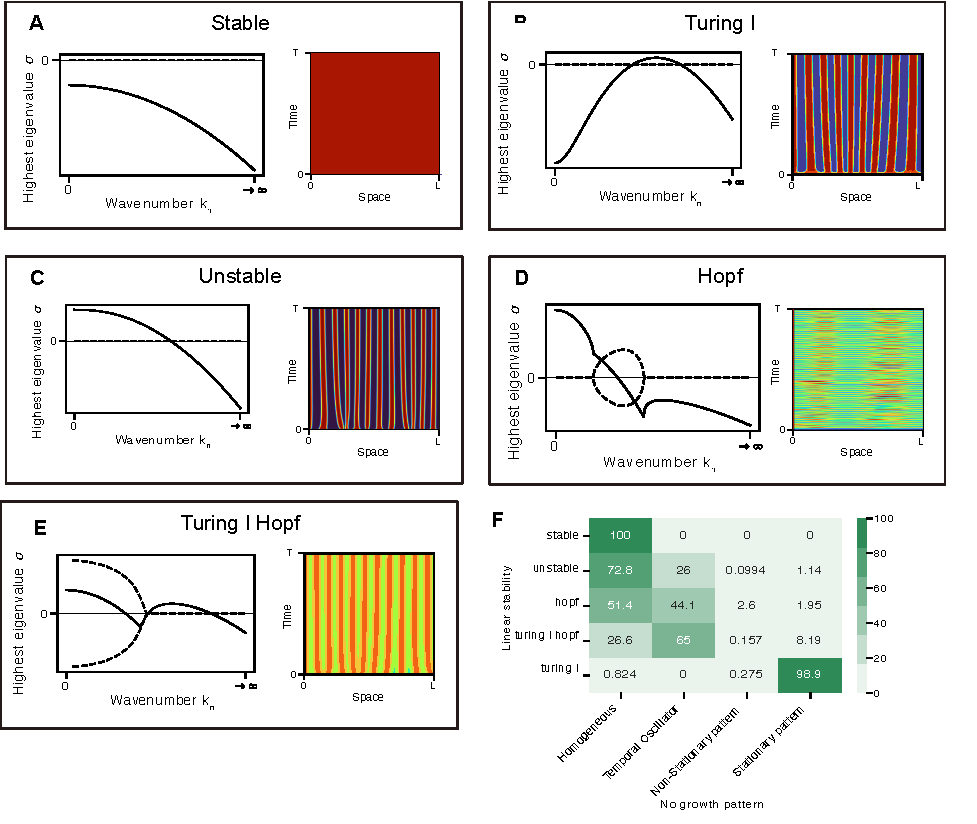
\includegraphics[width=1\textwidth]{figures/dispersion} % The name of your image file; assumes it is in the same directory as your .tex file
    \caption{\textbf{Relationship between dispersion relation and numerical solutions in mono-stable systems.} \textbf{(A-E)} Examples of a dispersion relation (left) and a resulting numerical solution (right) for Stable, Turing I, Unstable, Hopf, and Turing I Hopf. \textbf{(F)} Confusion matrix linking LSA output (rows) and numerical pattern outcome (columns). Numbers show the percentage of solutions across the LSA output rows.}
    \label{fig:dispersions} % A label for referencing this figure later in the document
\end{figure}


\subsection{Multistability}

Multi-stable systems are another case where linear stability analysis (LSA) fails to predict pattern formation.  In this section, we demonstrate how linear stability analysis (LSA) is neither sufficient 
nor necessary to predict Turing patterns in multi-stable system. In particular, we study in detail the dynamical behaviour of multi-stable systems during pattern formation, which will lead to the creation or breaking of the pattern.
The motivation behind this arises from the high degree of multistability exhibited by biological systems, especially in those systems with non-linearities and feedback loops, as occuring in biology or synthetic systems (see Eqs.~\ref{eq:turinghill})~\parencite{pham2020complexity, leite2009multistability}.

Using the two-node non-linear Turing topology (Eq.~\ref{eq:turinghill}), multi-stable solutions were identified by finding the steady states of the system using the Newton-Raphson method. These multi-stable solutions were then studied to understand how the patterning dynamics are affected in the presence of multiple steady-state solutions.
As in Section~\ref{nogrowth}, LSA was carried out to find multi-stable solutions and the Crank Nicholson algorithm was run to obtain the numerical solution of these.
Following the classical hypothesis used in the Turing literature, we expected stable and unstable systems to not produce patterns and equations fulfilling the Turing conditions to produce patterns.
Here, we present various examples of how this hypothesis can break in the presence of multistability.

Figure ~\ref{fig:multistability1} shows a case where diffusion-driven instability conditions are not required for Turing pattern formation.
The unstable state, having a dispersion relation with a peak below zero (Fig.~\ref{fig:multistability1}C), manages to form Turing patterns as it is attracted by the neighbouring Turing steady state.
It therefore produces a stationary pattern (Fig.~\ref{fig:multistability1}B), even though its dispersion relation does not predict so.
This trajectory is depicted in the phase diagram (Fig.~\ref{fig:multistability1}A) which shows the steady states along with the vector field to understand the potential trajectories of the system.
The phase diagram does not fully capture the dynamics as it describes the system without diffusion, while the dispersion relation and the numerical solution do consider diffusion.

\begin{figure}[H]
    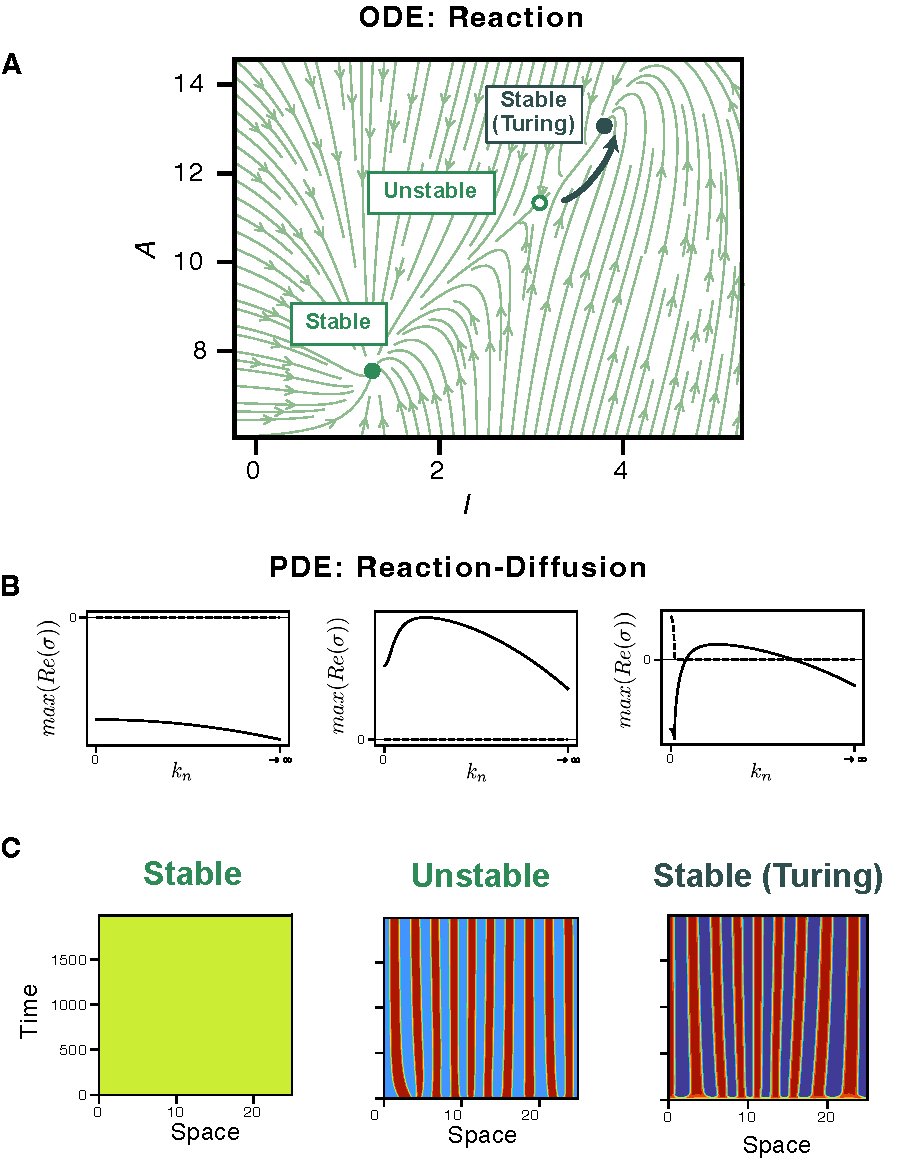
\includegraphics[width=1\textwidth]{figures/multistability1}

    \caption{\textbf{Stationary patterns with multistability.} \textbf{(A)} Phase diagram without diffusion illustrating three distinct steady states where the derivative is zero: stable, unstable, and stable (Turing). These steady states are represented within a parameter space defined by the two concentrations $A$ and $I$. The vector field, indicated by light green arrows, shows the direction of the derivatives of the system at various points in the parameter space. A hand-drawn trajectory is also shown (dark green arrow), demonstrating how the unstable state may evolve into the Turing state. \textbf{(B)} Dispersion relation showing each type of state. \textbf{(C)} Numerical solutions of the three steady states with diffusion, where the unstable state unexpectedly produces a Turing-like stationary pattern. }
    \label{fig:multistability1}
\end{figure}
%TODO make font smaller in figure


Next, we present a case where LSA incorrectly predicts stationary pattern formation.
Figure ~\ref{fig:multistability2} shows an ephemeral or transient pattern that occurs in the unstable and Turing regimes.
The Turing pattern initially develops in the vicinity of the Turing steady state.
As the spatial heterogeneity is amplified and settles, it gets attracted by the stable steady state leading to the disruption of the pattern.
This type of transient pattern behaviour has also been recently reported in~\cite{Krause2023}.

\begin{figure}[H]
        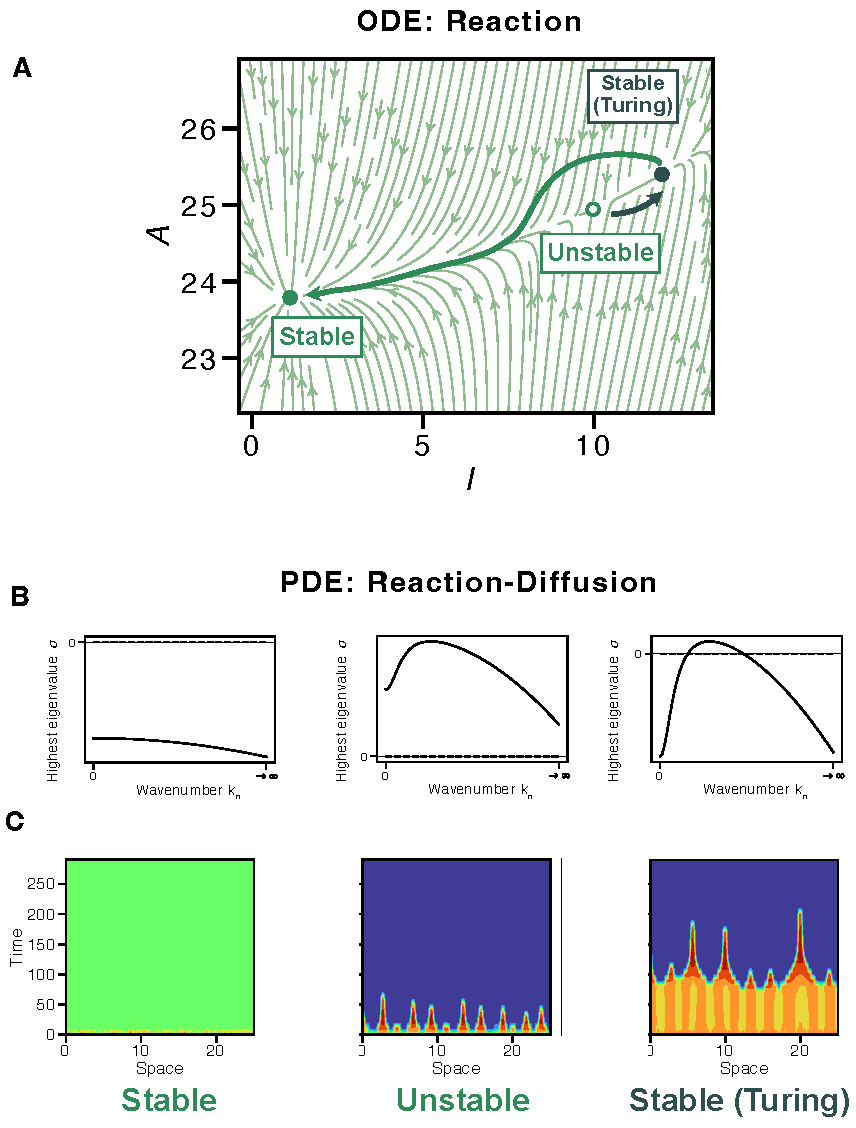
\includegraphics[width=1\textwidth]{figures/multistability2} % The name of your image file; assumes it is in the same directory as your .tex file
    \caption{\textbf{Ephemeral patterns with multistability.} \textbf{(A)} Phase diagram without diffusion illustrating three distinct steady states where the derivative is zero. The hand-drawn trajectory (dark green arrow) shows an unstable state evolving into a stable (Turing) and a regular stable (non-Turing) state, indicated by thick black and green arrows, respectively. \textbf{(B)} Dispersion relation showing each type of state. \textbf{(C)} Numerical solutions of three steady states with diffusion. Unstable and Turing states produce temporary periodic stationary patterns that then disappear and become spatially homogeneous solutions.}
    \label{fig:multistability2} % A label for referencing this figure later in the document
\end{figure}

Other interesting examples can be found, for example, where an unstable state is surrounded by two Turing states. This unstable state leads robustly to a Turing pattern (Fig.~\ref{sup_fig4}A).
Additionally, in some cases, the unstable system settles into Turing, but the Turing system gets pulled by the stable attractor (Fig. ~\ref{sup_fig4}B). Additionally, some systems even exhibit three solutions which are homogeneous in time and space (Fig.~\ref{sup_fig4}C). In this case, it would be worth investigating earlier time points with more resolution, as a pattern might appear then.
Similar interactions occur with multistability involving Turing I-Hopf solutions, which are mentioned in the following sections (Fig.~\ref{sup_fig4}D).




\section{Biological features: absorbing boundaries and growth}
As shown above, both numerical solutions and multistability can break the preconception that only classical Turing I systems can produce stationary periodic patterns.
Here, we look deeper into how other aspects linking the theory closer to the biological reality can also break this preconception.
In particular, we look at how adding absorbing boundaries and growth lead to a reaction-diffusion system may induce or break patterning.
This particular direction was inspired by experiments described in~\parencite{Oliver2023}, where growing bacterial colonies in agar are used as a platform to engineer Turing patterns using synthetic gene circuits (see Fig.~\ref{fig1}A.

The parameter space was explored using simulations, classified as  (1) no-growth and reflective boundaries, (2) no-growth and absorbing boundaries, and finally (3) growth and absorbing boundaries. This way we can understand separately the effects of absorbing boundaries and growth in a synthetic system such as~\parencite{Oliver2023}
Again, all these parameter sets have only a single steady state to ensure patterning effects are due to boundaries and growth, and not due to multistability.

When absorbing boundaries or growth are added, periodic patterns are potentially created, disrupted, or remain the same. The Sankey diagram in Fig~\ref{fig:boundariesgrowth}A shows how this system can transition when absorbing boundaries and growth are introduced.
As explained in the methods section below (see Section ~\ref{classification}), the classification previously used cannot be used for absorbing boundary conditions as these prevent the pattern from being completely homogeneous or stationary.  %TODO ref classification. %TODO add letter to image
Therefore, a different type of classification has to be used for reflective and absorbing boundary conditions. For reflective boundary conditions we classify patterns into (1) homogeneous, (2) temporal oscillators, (3) non-stationary patterns and (4) stationary patterns (see Section ~\ref{numerical_classification1}). For absorbing boundary conditions we classify patterns into (1) homogeneous, (2) boundary effect, (3) weak pattern, (4) intermediate pattern, and (5) strong pattern (see Section ~\ref{numerical_classification2}).
Although the classification outputs cannot be directly compared, this confusion matrix is useful to identify interesting cases:
If absorbing boundary conditions had no effect, we would expect homogeneous and temporal oscillator categories in the y-axis to become no pattern, homogeneous, or boundary effect.
Additionally, we would expect stationary patterns to become strong patterns.
This is commonly the case as seen by the thicker lines in~\ref{fig:boundariesgrowth}A, which shows boundaries do not often affect the pattern.
However, some exceptions are present which are further studied in Fig~\ref{fig:boundariesgrowth}B.

In particular, we observe systems where an absorbing boundary condition makes a homogeneous solution become a non-stationary pattern. Additionally, absorbing boundary conditions can turn a temporal oscillator into a stationary pattern. Finally, by adding growth, a non-stationary pattern can be stabilized into a growing stationary pattern.
\begin{figure}[H]
    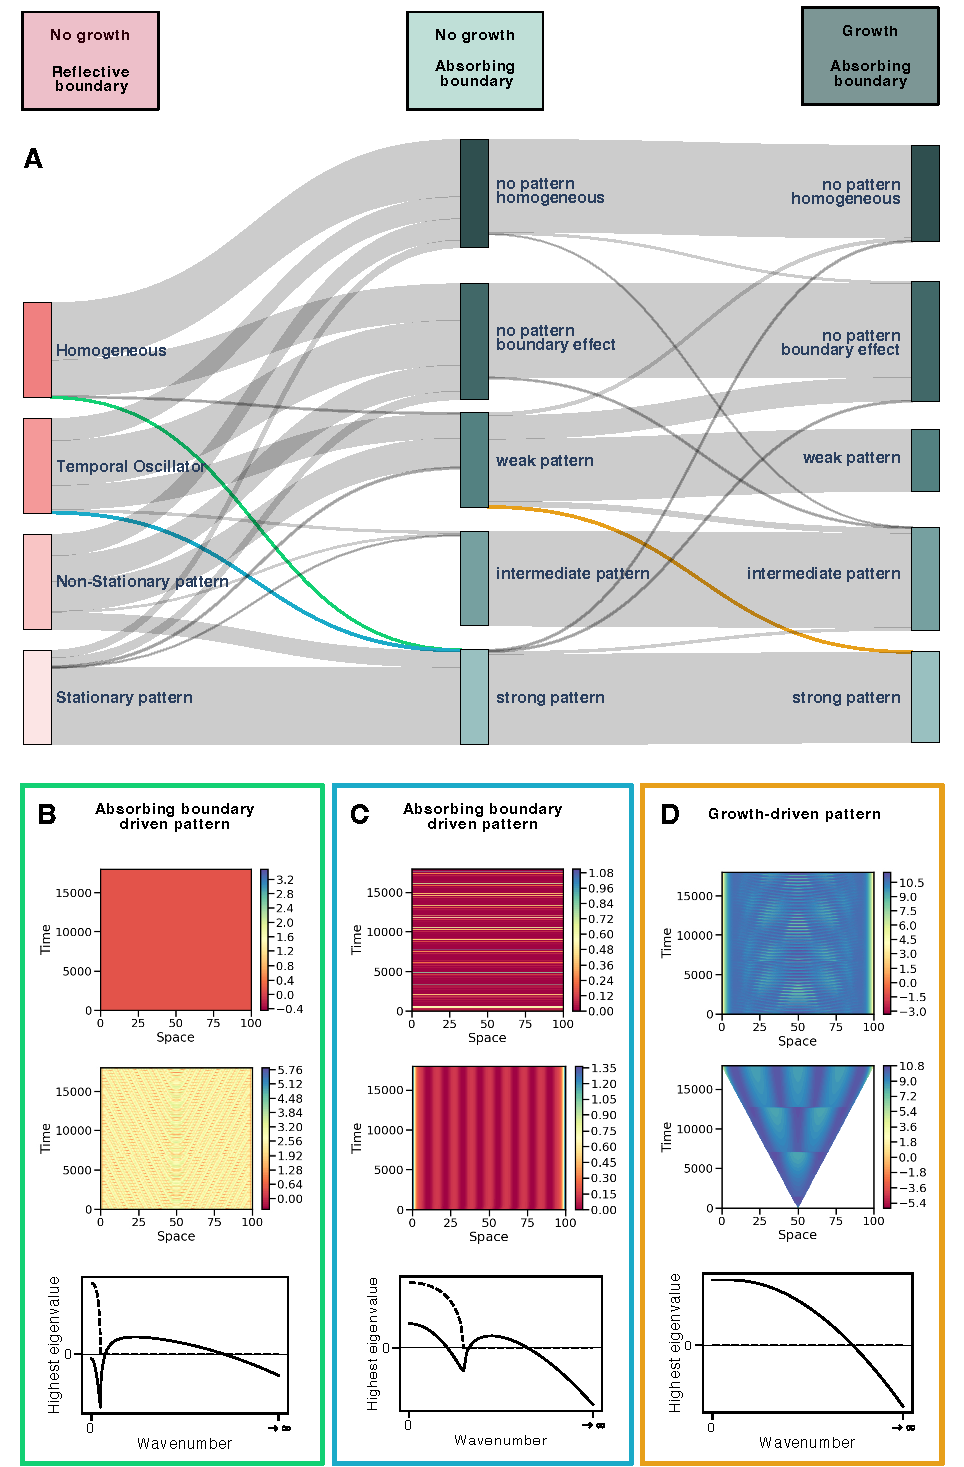
\includegraphics[width=1\textwidth]{figures/boundaries_growth} % The name of your image file; assumes it is in the same directory as your .tex file
    \caption{a}
    \label{fig:boundariesgrowth} % A label for referencing this figure later in the document
\end{figure}